\documentclass[12pt]{article}

\usepackage{amsmath}
\usepackage{amssymb}
\usepackage{pgfplots}
\usepackage{mathtools}
\usepackage{indentfirst}

\usetikzlibrary{angles, quotes}

\pgfplotsset{compat=newest}

\title{Complex Analysis}
\author{Linxuan Ma}

\begin{document}
	\maketitle
	
	\newcommand{\mo}[1]{\lvert #1 \rvert}
	\newcommand{\mos}[1]{\lvert #1 \rvert^2}
	\newcommand{\RR}{\mathbb{R}}
	
	\abstract{Convex analysis is the domain of mathematics that investigates functions of complex numbers. Despite its frequent occurrence in applied science, IB Mathematics seems to decide on not covering anything other than "haha $i^2$ is $-1$", so here's my attempt at creating notes for it after binging an entire semester of complex analysis in one night and getting sick immediately the next day due to sleep deprivation. Balanced IB life.}
	
	\section{Fundamentals}
	A complex number $z \in \mathbb{C}$ is a number of the form $$a + bi$$ where $a$ and $b$ are both real numbers.
	
	\subsection{Definitions}
	The imaginary number $i$ is defined as $\sqrt{-1}$. Due to its equivalence with $\sqrt{1}$, $i$ obeys all arithmetic laws that apply to root terms. Similarly, it coerces into $-1 \in \RR$ in the case of $i^2$.
	
	Due to the encapsulation of $z \in \mathbb{C}$ over real numbers $a$ and $b$, a complex function $f: \mathbb{C} \to \mathbb{C}$ is isomorphic to $g: \RR^2 \to \RR^2$. Trivially, by decomposition we obtain
	\begin{gather*}
		\Re: \mathbb{C} \to \RR \\
		\Im: \mathbb{C} \to \RR
	\end{gather*}
	corresponding to retrieving real components $a$ and $b$.
	
	Deriving from $z \in \mathbb{C}$'s correspondence to a vector $\vec{z} \in \RR$, the representation of a 2-dimensional coordinate can be concluded from $x$:
	
	\begin{equation*}
		\begin{bmatrix}
			\Re(z) \\ \Im(z)
		\end{bmatrix}
	\end{equation*}
	
	From such geometric representation, further vector-like properties can be defined (conjugate, modulus and argument) for $z \in \mathbb{C}$ with real part $a$ and imaginary part $b$:
	
	\begin{gather*}
		\overline{z} = a - bi \\
		\mo{z} = \sqrt{a^2 + b^2} \\
		\arg z = \arctan \frac{b}{a}
	\end{gather*}
	
	Note the isomorphism of the modulus-argument pair with the standard $a + bi$ form under the domain $-\pi < \theta \leq \pi$ for argument. In the remaining portion of this note, a complex number may take any of the following form:
	
	\begin{enumerate}
		\item Regular form: $a + bi$ where $a, b \in \RR$
		\item Tuple form (equivalent to $a + bi$): $(a, b)$
		\item Polar form (modulus $r$ and argument $\theta$): $r(cos \theta + i \sin \theta)$
	\end{enumerate}
	
	\subsection{Complex Arithmetic}
	
	Trivially, due to the nature of square roots:
	
	\begin{gather*}
		(a, b) + (c, d) = (a + c, b + d) \\
		(a, b) - (c, d) = (a - c, b - d) \\
		(a, b) * (c, d) = (ac - bd, ad + bc) \\
		\frac{(a, b)}{(c, d)} = \frac{(a, b)(c, -d)}{(c, d)(c, -d)}
	\end{gather*}
	
	Conjugation is distributive over addition, subtraction, multiplication and division:
	
	\begin{gather*}
		\overline{z + w} = \overline{z} * \overline{w} \\
		\overline{z - w} = \overline{z} * \overline{w} \\
		\overline{z * w} = \overline{z} * \overline{w} \\
		\overline{\left(\frac{z}{w}\right)} = \frac{\overline{z}}{\overline{w}}
	\end{gather*}
	
	It is clear that the complex conjugation $z \to \overline z$ is an automorphism of $\mathbb{C}$ (an isomorphic endofunctor).
	
	Trivially, $z * \overline z \in \RR$.
	
	Rules regarding the polar representation can be trivially obtained via substitution of definitions:
	
	\begin{gather*}
		\mo{z * w} = \mo{z} * \mo{w} \\
		\arg(z * w) = \arg z + \arg w
	\end{gather*}
	
	Modulus can be viewed as the distance of the represented point to the origin, and thereby the rule:
	
	\begin{gather*}
		\mo{z * w} \leq \mo{z} * \mo{w}
	\end{gather*}
	
	\subsection{Simple Applications}
	
	The following section explores rudimentary applications we can derive from the previously covered rules of complex numbers.
	
	\subsubsection{Magma of Sums of Squares Under Multiplication}
	
	Consider the number theory problem:
	\begin{center}
		Which integers are sums of two squares?
	\end{center}
	
	With complex numbers, we realize that the integers that are the sum of two squares form a magma under multiplication.
	\\\\
	\textbf{Proof.} There exists an rearrangement of terms in a product of sums of 2 squares such that: $$(a^2 + b^2)(c^2 + d^2) \to (ac - bd)^2 (ad + bc)^2$$
	The above transformation is derived from the complex number rules related to complex modulus:
	
	\begin{gather*}
		a^2 + b^2 = \mos{a + ib} \\
		c^2 + d^2 = \mos{c + id}
	\end{gather*}
	Therefore $(a^2 + b^2)(c^2 + d^2)$ can be written as:
	
	\begin{align*}
		  & (a^2 + b^2)(c^2 + d^2) \\
		= & \mos{(a + ib)(c + id)} \\
		= & \mos{ac - bd + i(ad + bc)} \\
		= & (ac - bd)^2 + (ad + bc)^2
	\end{align*}
	 
	Extending from the proof above, consider two given sum of squares:
	
	\begin{gather*}
		5 = 1^2 + 2^2 \\
		13 = 2^2 + 3^2
	\end{gather*}
	
	By multiplication we obtain: $$5 * 13 = 65$$
	
	Note that $65$ can also be represented as different sums of two squares: $1^2 + 8^2 = 4^2 + 7^2 = 65$. By writing the constituent of $5$ and $13$ as complex modulus, we obtain:
	
	\begin{gather*}
		\mos{1 + 2i} = 5 \\
		\mos{2 + 3i} = 13
	\end{gather*}
	
	By multiplying $1 + 2i$ and $2 + 3i$ and conjugating one of them, we obtain:
	
	\begin{gather*}
		(1 + 2i)(2 + 3i) = -4 + 7i \\
		(1 + 2i)(2 - 3i) = 8 + i
	\end{gather*}
	corresponding to the other two solution $1^2 + 8^2 = 65$ and $4^2 + 7^2 = 65$.
	
	\subsubsection{Pythagorean Triples}
	
	Another application of complex arithmetic relates to the Pythagorean theorem, easily generating a set of Pythagorean triples from complex numbers. Consider the Pythagorean theorem of edge $a, b, c$ where $c \leq a + b$ in a right triangle: $$a^2 + b^2 = c^2$$
	
	Consider the modulus of an arbitrary complex number with integer real and imaginary parts, i.e. $a + bi$ where $a, b \in \mathbb{Z}$, then its modulus can be expressed as a single square root of an integer. Therefore, the modulus of the square of any $a + bi$ of integer coordinate is an integer:
	\begin{align*}
		\mo{a + bi} &= \sqrt{a^2 + b^2} \\
		(a + bi)^2 &= a^2 - b^2 + (2ab)i  \\
		\mo{(a + bi)^2} &= \mo{a + bi} * \mo{a + bi} \\
		& = a^2 + b^2
	\end{align*}
	
	Therefore, we obtain a generalized formula of the Pythagorean triples over the complex plane for any integer substitution of $a$ and $b$:
	\begin{align*}
		a &= a^2 - b^2 \\
		b &= 2ab \\
		c &= a^2 + b^2
	\end{align*}
	
	
	\subsubsection{Quaternions}
	
	A feasible expansion of the complex number system into $\RR^3$ has yet to be proposed. However, there exists a $\RR^4$ expansion, the quaternions, of the complex plane.
	
	In the quaternion system, a complex number $a + bi$ is expanded into $a + bi + cj + dk$, where the multiplication of $i$, $j$ and $k$ is not communicative:
	\begin{gather*}
		i^2 = j^2 = k^2 = ijk = -1 \\
		ij = k = -ji \\
		jk = i = -kj \\
		ki = j = -ik
	\end{gather*}
	
	Similar to finding the inverse of a complex number $a + bi$ (multiplying nominator and denominator by its conjugate):
	$$\frac{1}{a + bi} = \frac{a - bi}{a^2 + b^2}$$
	, there also exists an inverse for a quaternion:
	$$\overline{a + bi + cj + dk} = a - bi - cj - dk$$
	
	The product of a quaternion with its conjugate is:
	\begin{align*}
		z\overline{z} = a^2 + b^2 + c^2 + d^2
	\end{align*}
	
	Note that the cross terms (such as $bcij$ and $bcji$) in the above equation vanish due to the non-commutativity ($ij$ = $-ji$).
	
	The inverse of a quaternion can thus be found:
	$$\frac{1}{a + bi + cj + dk} = \frac{a - bi - cj - dk}{a^2 + b^2 + c^2 + d^2}$$
	
	All none-zero quaternions have inverses, similar to complex numbers.
	
	\section{Roots}
	
	Finding roots of complex numbers is significant in complex analysis. The square root of $x \in \RR$ can be represented as a complex number, such as:
	\begin{align*}
		\sqrt{10} &= \sqrt{10} + 0i \\
		\sqrt{-5} &= \sqrt{5}i
	\end{align*}
	
	Due to the complications of working with the cartesian form of complex numbers in multiplication and division, the majority of calculations below feature $z \in \mathbb{C}$ in the exponential form, namely $re^{i\theta}$. This trivially corresponds to the polar form $r(\cos \theta + i\sin \theta)$ as dicussed previously.
	
	The conversion from cartesian to polar can be roughly described as (neglecting the domain restrictions):
	\begin{align*}
		r &= \mo{z}
	\end{align*}
	
	\subsection{Geometric Interpretation of Multiplication}
	
	To better represent multiplication over the complex plane, we shall express multiplication in complex number's polar 
	\begin{center}
		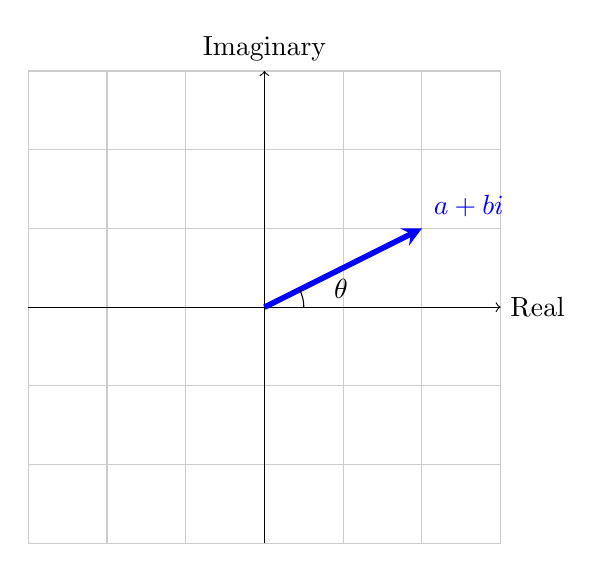
\begin{tikzpicture}
			\coordinate (o) at (0, 0);
			\coordinate (a) at (1, 0);
			\coordinate (b) at (2, 1);
		
			\draw[thin,gray!40] (-3, -3) grid (3, 3);
			\draw[->] (-3, 0)--(3, 0) node[right]{Real};
			\draw[->] (0, -3)--(0, 3) node[above]{Imaginary};
			\draw[line width=2pt,blue,-stealth](0, 0)--(2, 1) node[anchor=south west]{$a + bi$};
			
			\pic [draw, -, "$\theta$", angle eccentricity=2] {angle = a--o--b};
		\end{tikzpicture}
	\end{center}
	
	From the above illustration we can conclude that:
	\begin{align*}
		z &= a + bi \\
		r &= \mo{z} \\
		x &= r * \cos \theta \\
		y &= r * \sin \theta \\
		\frac{y}{x} &= \tan \theta
	\end{align*}
	
	Consider the set of complex numbers $S^1$ ($S$ for sphere, and $1$ for 1-dimensional) whose modulus is 1. This forms a group over multiplication, i.e:
	\begin{gather*}
		\forall z_1, z_2 \in S^1,\ \mo{z_1} = \mo{z_2} = 1 \\
		z_1 * z_2 = 1 \\
		\mo{z_1^{-1}} = 1
	\end{gather*}
	
	Note that every complex number can be written in $r * z_i$ for a specific $z_i \in M$. In other words, there exists a unique isomorphism between any non-zero complex number and a $z_i$ scaled by a constant $r$: $$a + bi \cong r * z_i \ \text{for}\ a, b, r \in \RR,\ z_i \in S^1$$
	
	
	$\mathbb{C}^*$ (non-zero complex number) is the product of $\RR_{>0} \times S^1$, and thus $$r_1 e^{i\theta_1} * r_2 e^{i\theta_2} = r_1r_2e^{i(\theta_1 + \theta_2)}$$
	can be easily deduced. This also hints complex number's proficiency at representing rotations of $\RR^2$ (and therefore the existence of quaternions to describe rotations in $\RR^3$).
	
	\textbf{Warning:} When multiplying complex numbers on a computer, care must be taken to map the polar angles to $(-\pi, \pi]$ when converting from cartesian form to polar form.
	
	\subsection{Square Root of $z \in \mathbb{C}$}
	
	With the aforementioned geometric representation of complex multiplication, $\sqrt{z}$ for $z \in \mathbb{C}$ can be trivially obtained as:
	\begin{gather*}
		\sqrt{z} = \sqrt{re^{i\theta}} = \sqrt{r}e^{i\frac{\theta}{2}}
	\end{gather*}
	
	There exists two solutions for the square root of a complex number. Therefore, in order to preserve continuity, we realize that $\sqrt{e^{i\pi}}$ and $\sqrt{e^{-i\pi}}$ should be equal, yet the continuity of the square root function insists that:
	\begin{align*}
		\sqrt{e^{i\pi}} &= i \\
		\sqrt{e^{-i\pi}} &= -i
	\end{align*}
	
	There exists no solution to this inequality; however, since we normally only consider the domain $(-\pi, \pi]$, this inconsistency is not \textit{that} significant.
	
	\subsection{$n$-th Root of $z \in \mathbb{C}$}
	
	Consider the complex number $3 + 4i$ and its fifth root. Its modulus is $5$, and therefore $\mo{\sqrt[5]{3 + 4i}} = 5$. Interestingly, there exists multiple solutions for $\arg \sqrt[5]{3 + 4i}$, as:
	$$\frac{\theta}{5},\ \frac{\theta + 2\pi}{5},\ \frac{\theta + 4\pi}{5},\ \dots$$
	are all valid solutions to $\arg \sqrt[5]{3 + 4i}$ (since the original $3 + 4i$ can also be represented with argument of $\theta$, $\theta + 2\pi$, $\theta + 4\pi$, etc). This behavior is distinct from taking an odd root of a real number, and therefore introduces complications.
	
	Interestingly, the argument of the fifth root of $3 + 4i$, when plotted on the complex plane, forms a pentagon:
	\begin{center}
	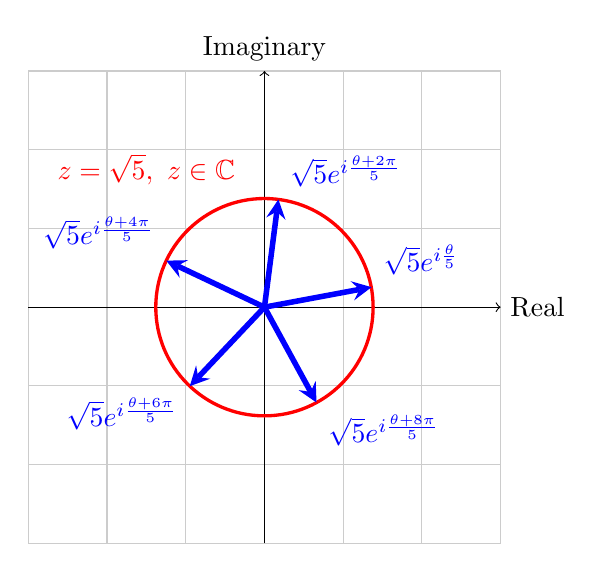
\begin{tikzpicture}
		\coordinate (o) at (0, 0);
		\coordinate (a) at (1, 0);
		\coordinate (b) at (2, 1);
	
		\draw[thin,gray!40] (-3, -3) grid (3, 3);
		\draw[->] (-3, 0)--(3, 0) node[right]{Real};
		\draw[->] (0, -3)--(0, 3) node[above]{Imaginary};
		
		\draw[red, very thick] (0, 0) circle [radius=1.380];
		\node[red] at (-1.5, 1.75) {$\mo{z} = \sqrt{5},\ z \in \mathbb{C}$};
		
		\draw[line width=2pt, blue, -stealth](0, 0)--(1.36, 0.254) node[anchor=south west]{$\sqrt{5}e^{i\frac{\theta}{5}}$};
		\draw[line width=2pt, blue, -stealth](0, 0)--(0.177, 1.369) node[anchor=south west]{$\sqrt{5}e^{i\frac{\theta + 2\pi}{5}}$};
		\draw[line width=2pt, blue, -stealth](0, 0)--(-1.247, 0.591) node[anchor=south east]{$\sqrt{5}e^{i\frac{\theta + 4\pi}{5}}$};
		\draw[line width=2pt, blue, -stealth](0, 0)--(-0.948, -1.003) node[anchor=north east]{$\sqrt{5}e^{i\frac{\theta + 6\pi}{5}}$};
		\draw[line width=2pt, blue, -stealth](0, 0)--(0.661, -1.211) node[anchor=north west]{$\sqrt{5}e^{i\frac{\theta + 8\pi}{5}}$};
	\end{tikzpicture}
	\end{center}
	
	This pattern generalizes across the $n$-th roots of a complex number, forming a regular $n$-sided polygon around the origin with radius of $\sqrt[n]{\mo{z}}$.
	
	Therefore, any $z \in \mathbb{C}$ has $n$-th root. Inductively, the polynomial $z^n - a$ always has a root.
	
	For more complicated polynomials there also exists a complex root,  but won't be proved in this section: $$z^n + a_{n-1}z^{n - 1} + a_{n - 2}^2z^{n - 2} + \dots + a_1z + a_0 = 0$$
	
	$\mathbb{C}$ is therefore "algebraically closed".
	
	Recall the formula:
	\begin{align*}
		\cos 2\theta &= \cos^2 \theta - sin^2 \theta \\
		\cos 3\theta &= \cos^3 \theta - 3\cos \theta \sin^2 theta
	\end{align*}
	and so on. The above formula can be obtained by the binomial theorem:
	\begin{gather*}
		\cos(n\theta) + i\sin(n\theta) = (\cos \theta + i \sin\theta)^n
	\end{gather*}
	
	The above formula correspond to the the geometric interpretation of complex multiplication: addition of the arguments corresponds to multiplication of the numbers (given that modulus is $1$).
	
	The right hand side can be expanded via the binomial theorem, resulting in:
	\begin{gather*}
		\cos^n \theta + in\cos^{n - 1}\theta\sin\theta - \binom{n}{2} \cos^{n - 2}\theta \sin^2 \theta + \dots
	\end{gather*}
	which, after applying the above to $\Re$, will equal to the original $\cos(n\theta)$.
	
	\section{Exp, Log and Trigonometry}
	
	The exponential function can be defined as a power series that converges:
	$$\exp(z) = 1 + z + \frac{z^2}{2!} + \frac{2^3}{3!} + \dots$$
	
	If a series of complex numbers $a_0 + a_1 + a_2 + \dots$ is convergent, then $\Re(a_0) + \Re(a_1) + \dots$ and $\Im(a_0) + \Im(a_1) + \dots$ also converges due to $\mo{\Re(z)} \leq \mo{z}$ and $\mo{\Im(z)} \leq \mo{z}$.
	
	\subsection{The Exponential Function}
	Properties of the exponential function includes:
	\begin{gather*}
		\exp(z_1 + z_2) = \exp(z_1) * \exp(z_2)
	\end{gather*}
	which can be proven with:
	\begin{align*}
		\sum_{n=0}^\infty \frac{(z_1 + z_2)^n}{n!} &= \sum_{n, m=0}^\infty \frac{\binom{n}{m}z_1^m z_2^{n - m}}{n!} \\
		&= \sum_{n, m=0}^\infty \frac{z_1^m}{m!}*\frac{z_2^{n-m}}{(n-m)!} \\
		&= \sum_{n, m=0}^\infty \frac{z_1^m}{m!}*\frac{z_2^n}{n!} \\
		&= \exp(z_1) * \exp(z_2)
	\end{align*}
	
	Defining $z \in \mathbb{C}$ as $z = a + bi$, $e^z = e^{a + bi} = e^a*e^{bi}$. Note that the left section $e^a \in \RR$, while $e^{bi} \in \mathbb{C}$. We can rewrite this as:
	\begin{align*}
		\exp(bi) &= 1 + bi + \frac{b^2i^2}{2!} + \frac{b^3i^3}{3!} + \dots \\
		&= 1 + bi - \frac{b^2}{2!} - \frac{-b^3i}{3!} + \frac{b^4}{4!} + \dots
	\end{align*}
	
	Note that the series $1,\ -\frac{b^2}{2!},\ \frac{b^4}{4!},\ \dots$ is just the series for $\cos(b)$, while the series $bi,\ -\frac{b^3i}{3!},\ \frac{b^5i}{5!},\ \dots$ is the series for $i * \sin(b)$.
	
	Therefore, Euler's identity can be deduced from the above equation: 
	\begin{align*}
		e^{i\theta} &= \cos \theta + i \sin \theta \\
		e^{i\pi} &= -1 \\
		e^{2i\pi} &= 1 \\
		e^{2ni\pi} &= 1,\ n \in \mathbb{Z}
	\end{align*}
 		
 	Exponentials can also be viewed as a homomorphism of groups (note that the mapping is surjective but not injective): $$\exp(z_1 + z_2) = \exp(z_1)\exp(z_2)$$
 	from complex numbers under addition to complex numbers under multiplication (in polar coordinates): $$\mathbb{C} \xrightarrow{\exp} \mathbb{C}^*$$

	The above is satisfied if the modulus of the object being mapped is non-zero. In addition, observe that:
	\begin{align*}
		r(\cos \theta + i\sin \theta) &= r * \exp(i\theta) \\
		&= \exp(\ln r) * \exp(i\theta) \\
		&= \exp(\ln r + i\theta)
	\end{align*}
	therefore the homomorphism is satisfied for $r \neq 0$.
	
	Incidentally, there also exists a homomorphism of real numbers $\RR$ under addition to $\RR$ under multiplication that is injective yet not surjective (trivial).
	
	\subsection{The Logarithm Function}
	
	The $\ln$ function is the inverse of the exponential function e.g. solving for $a$ and $b$ in $\exp(a + bi) = z$ becomes $a + bi = \ln z$. Since the polar representation of $a + bi$ is $r(\cos \theta + i\sin \theta)$, it can be deduced that:
	\begin{align*}
		\exp(a) &= r = \mo{z} \\
		\theta &= \arg z
	\end{align*}
	
	Note that $\ln(z)$ is not unique (only defined up to multiples of $2\pi i$). The logarithm function can't be defined continuously for all non-zero complex numbers (due to the ambiguity in the argument of the complex number):
	$$z_1^{z_2} = \exp(z_2 * \ln(z_1))$$
	is only well-defined when:
	\begin{enumerate}
		\item $z_1 > 0$ and $z_1 \in \RR$ (trivial)
		\item $z_2 \in \mathbb{Z}$ (ambiguity is unimpactful as $z_1^{z_2} = 1$)
	\end{enumerate}
	
	\subsection{Trigonometric Functions}
	
	The $\cos$ function and $\sin$ function are just special cases for the exponential function:
	\begin{align*}
		e^{iz} &= \cos z + i\sin z \\
		e^{-iz} &= \cos z - i\sin z \\
		\frac{e^{iz} + e^{-iz}}{2} &= \cos z
	\end{align*}
	
	The same conclusion is arrived for defining $\cos$ as the power series derived from the definition (in series form) of the exponential function.
	
	Similarly: $$\frac{e^{iz} + e^{-iz}}{2} = \cos z$$
	
	In addition, identities of the trigonometric functions follow the identity of the exponential function:
	\begin{align*}
		\cos(\theta_1 + \theta_2) &= \cos \theta_1 \cos \theta_2 - \sin \theta_1 \sin \theta_2 \\
		\exp(z_1 + z_2) &= \exp(z_1) * \exp(z_2) \text{ (substitution)}
	\end{align*}
	
	Note that the $\sin$ and $\cos$ functions are defined over the entire complex plane due to its correspondence with Euler's identity.
	
	\subsection{Applications of Complex Trigonometry}
	
	Due to the flexibility of trigonometric functions in the complex plane, there are numerous applications of it. The following section lists a few simple and significant ones.
	
	\subsubsection{Differential Equation}
	
	Consider the linear differential equation: $$a\frac{d^2y}{dx^2} + b\frac{dy}{dx} + cy = 0$$
	With complex numbers, the above can be solved trivially:
	\begin{align*}
		y &= e^{\lambda x} \\
		a\lambda^2e^{\lambda x} + b\lambda e^{\lambda x} + ce^\lambda &= 0 \\
		a \lambda^2 + b\lambda + c &= 0
	\end{align*}
	
	$\lambda$ can be solved with a simple quadratic equation. Consider the example: $$\frac{d^2 y}{dx} + 2\frac{dy}{dx} + 2y = 0$$
	By implementing the concept above, we obtain:
	\begin{align*}
		\lambda^2 + 2\lambda + 2 &= 0 \\
		\lambda = -1 \pm \sqrt{1^2 - 2} &= -1 \pm i \\
		\exp((1 + i)x),\ \exp((1 - i)x) &= y
	\end{align*}
	
	\subsubsection{Fourier Series}
	
	With a periodic function $f$: 
	\begin{gather*}
		f(x) = f(2\pi + x)
	\end{gather*}
	$f$ can be written as a sum of $sin$ and $cos$ functions (thus simplified with complex numbers):
	\begin{align*}
		f(x) &= \sum_{n > 0} a_n \sin(nx) + \sum_{n \geq 0} b_n \cos{nx} \\
		&= \sum_{n \in \mathbb{Z}} c_n e^{inx}
	\end{align*}
	
	\subsection{Tangent of $z$}
	
	The regular difinition for the trigonometric function $\tan$ is $\sin$ divided by $\cos$:
	\begin{gather*}
		\tan z = \frac{\sin z}{\cos z}
	\end{gather*}
	
	Due to Euler's indetity, $\tan$ can be represented as:
	\begin{gather*}
		\tan z = \frac{1}{i} * \frac{e^{iz} - e^{-iz}}{e^{iz} + e^{-iz}}
	\end{gather*}
	
	Except near the real axis, the tangent function is almost constant around $\tan z = i$.
	
\end{document}